%-------------------------
% Rover Resume - Base Template
% Link: https://github.com/subidit/rover-resume
%
% Shows code for various formatting options for different resume sections.
% Education and Projects have single-line headers; while Experience uses double-line.
% Some formatting codes are kept inline; consider \newcommand{cmd}{def}.
% Excludes hyperref and icons for readability; MVP version.
% Explore other templates for more options.
% Mix and match as desired. Be consistent with headers and sub-headers.
%------------------------

\documentclass[11pt]{article} % fontsize 10pt/11pt/12pt

\usepackage[margin=1in, a4paper]{geometry}
\setcounter{secnumdepth}{0} % remove section numbering
\usepackage{titlesec}
\usepackage{tikz} % Gói để vẽ khung hình thẻ
\usepackage[hidelinks]{hyperref} % Tùy chọn hidelinks sẽ ẩn khung viền và giữ màu đen cho chữ %
\titlespacing{\subsection}{0pt}{*1.5}{*0.5} % remove vertical spacing above and below
\titlespacing{\subsubsection}{0pt}{*0.5}{*0.5}
\titleformat{\section}{\large\bfseries\uppercase}{}{}{}[\titlerule]
\titleformat*{\subsubsection}{\large\itshape}
\usepackage{enumitem}
\setlist[itemize]{noitemsep,left=0pt .. \parindent}
\pagestyle{empty} % remove page number
\pdfgentounicode=1



\begin{document}

\begin{center}
    % Dòng 1: Hình thẻ bên trái và Tên bên phải
    \begin{minipage}[c]{0.2\textwidth}
        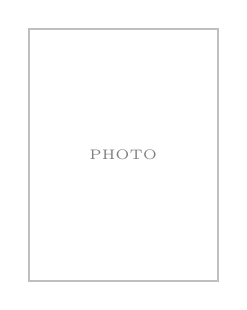
\begin{tikzpicture}
            % Khung hình chữ nhật 2.4cm x 3.2cm
            \draw[lightgray, line width=0.8pt] (0,0) rectangle (2.4, 3.2); %
            \node[text=gray, font=\tiny] at (1.2, 1.6) {PHOTO};
        \end{tikzpicture}
    \end{minipage}
    \hfill
    \begin{minipage}[c]{0.75\textwidth}
        \raggedleft
        {\Huge\bfseries Tan Kiet HONG} \\[5pt] %
        {\large Civil \& Geomechanics Engineer}
    \end{minipage}

    \vspace{15pt} % Khoảng cách giữa phần tên và thông tin liên hệ

    % Dòng 2: Các thông tin liên hệ căn giữa ở dưới (Sử dụng chữ thay cho Icon)
    \centering
    \small
    GitHub: \href{https://github.com/tankiet1907}{tankiet1907} \ $|$ \ 
    LinkedIn: \href{https://linkedin.com/in/tankiethong}{tankiethong} \ $|$ \ %
    Location: Grenoble, France \\[6pt] %
    
    Email: \href{mailto:hogtankit2001@gmail.com}{hogtankit2001@gmail.com} \ $|$ \ %
    Mobile: \href{tel:+33746502191}{(+33) 7 46 50 21 91} %
\end{center}

\section{Education}
%=================%
\subsection{Université Grenoble Alpes \hfill Sep 2025 - Present}
\subsubsection{Master 2: Geomechanics, Civil Engineering \& Risks \hfill \normalfont\textit{Grenoble, France}}
\begin{itemize}
    \item \textbf{Global Grade:} 13.47/20 (Admis). 
    \item \textbf{Key Coursework:} Quantitative Image Analysis for Mechanics (16/20), Durability and Vulnerability of Structures (15.8/20), Soil Dynamics and Nonlinear Site Response Analysis (15/20).
    \item \textbf{Thesis:} Numerical and experimental study of the thermo-hydro-mechanical (THM) behavior of concrete under severe accident conditions using a poro-mechanical approach.
\end{itemize}

\vspace{0.15cm}

\subsection{Ho Chi Minh University of Technology \hfill Sep 2019 - Jun 2024}
\subsubsection{Engineering Degree in Building \& Energy (PFIEV Program) \hfill \normalfont\textit{HCM City, Vietnam}}
\begin{itemize}
    \item \textbf{GPA:} 8.06/10 (3.5/4.0) $|$ \textbf{Rank:} 3/12 (Excellence Program).
    \item \textbf{Honors:} University Semester Scholarships for 4 consecutive years (2021-2024)
\end{itemize}

\section{Research \& Professional Experience}
%=================%
\subsection{M2 Research Intern / Thesis Student \hfill Feb 2026 - Present}
\subsubsection{3SR Laboratory, Université Grenoble Alpes \hfill Grenoble, France}
\begin{itemize}
    \item \textbf{Repository:} \href{https://github.com/tankiet1907/cast3m-m2internship}{github.com/tankiet1907/cast3m-m2internship}
    \item Investigating the thermo-hydro-mechanical (THM) behavior of concrete under severe accident conditions using a poro-mechanical approach.
    \item Developing and implementing numerical behavior models within the \textbf{Cast3M} finite element code using Gibiane.
    \item Utilizing probabilistic and statistical methods to conduct sensitivity analyses and optimize THM coupling parameters.
    \item Correlating numerical simulations with experimental data to validate predictive models for structural integrity.
\end{itemize}
\vspace{0.15cm}

\subsection{Structure Engineer (Full Time) \hfill Aug 2024 - Aug 2025}
\subsubsection{GBC Engineers Vietnam \hfill Ho Chi Minh City, Vietnam}
\begin{itemize}
    \item Prepared Finite Element Models (FEM) and structural models for rigorous mechanical analysis.
    \item Delivered structural calculations, analysis reports, and correspondence ensuring compliance with international standards (Eurocode, TCVN).
\end{itemize}

\vspace{0.15cm}

\subsection{Site Engineer (Internship) \hfill Jun 2023 - Aug 2023} % [cite: 73]
\subsubsection{Unicons Construction (Member of Coteccons Group) \hfill Binh Duong, Vietnam} 
\begin{itemize}
    \item \textbf{Project:} LEGO Manufacturing Vietnam Facility (Steel Structure specialist). 
    \item Managed construction progress and inspections; coordinated between subcontractors and consultants. 
    \item Completed additional internships at Hoa Binh Construction (2022) and SOL E\&C (2021).
\end{itemize}

\section{Projects}
%=================%
\subsection{Scientific Research: Fire-Resistant Steel Structures \hfill Sep 2023 - Dec 2023} 
\subsubsection{Ho Chi Minh City University of Technology \hfill Ho Chi Minh City, Vietnam}
\begin{itemize}
    \item Evaluated thermo-mechanical properties of steel at high temperatures per EUROCODE specifications. 
    \item Designed and verified fire-resistant structural elements (columns and beams) using advanced material models. 
\end{itemize}

\section{Certifications \& Awards}
%===============================%
\begin{itemize}
    \item \textbf{Third Prize, $36^{th}$ Loa Thanh Award (2024):} National award for the most prestigious graduation projects in civil engineering.
    \item \textbf{Third Prize in Physics (2018):} City Level Excellent Student Competition (Ho Chi Minh City).
    \item \textbf{Certificate of Merit:} Recognized as a "Very Good Student" for the 2021-2022 academic year.
\end{itemize}

\section{Skills \& Competencies}
%===========================%
\begin{description}[itemsep=0pt]
    \item[Technical:] Cast3M (Advanced), Finite Element Analysis (FEA), THM Coupling, Probabilistic Sensitivity Analysis.
    \item[Software:] LaTeX, Linux Mint, VS Code, Revit Structure, AutoCAD, ETABS, SAP2000, MS Office.
    \item[Languages:] Vietnamese (Native), English (Advanced - TOEIC: 935/990), French (Intermediate - TCF TP: 347/699, B1).
\end{description}

\section{Extracurricular Activities}
%===========================%
\begin{itemize}
    \item \textbf{Main Vocal:} Tet Festival of the Vietnamese Community in Grenoble. \hfill 2026
    \item \textbf{Main Vocal:} PFIEV Freshman Welcome Party (2023) and Journée de la Culture Française (2022). \hfill 2022 - 2023
    \item \textbf{Volunteer:} Supporting COVID-19 prevention work. 
    \item \textbf{Security Support:} Admissions Consulting Day (2022) and University Entrance Exam Support Program (2020). \hfill 2020 - 2022.
\end{itemize}

\vfill
\center{\footnotesize Last updated: \today}

\end{document}
